
Another harmful effect of the unstable propositions is
their effect on the duplicate detection mechanism of search algorithms.
To demonstrate that this effect is also reduced by ZSAE,
we measured the number of node generations
on the models resulted from vanilla SAE and ZSAE and successfully solved by
the planner (\refig{fig:ama1-visited}).
% ???
% Since the planner uses a blind search and the problem is unit-cost, all nodes under the solution depth are generated
% (note: mind the difference between evaluation, expansion, generation).
The plot supports our claim that
the randomness in the state encoding of vanilla SAE confuses the duplicate detection and
generates larger number of states compared to ZSAE.

\begin{figure}[htb]
 \centering
 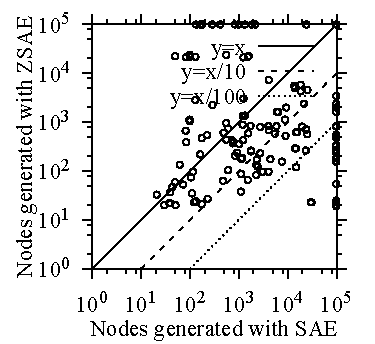
\includegraphics{img/static/gen.pdf}
 \caption{Double-logarithmic plot of the number of states generated by blind search
for the search space obtained from SAE and ZSAE with $N=64,100$ (all domains). 
Unsolved instances are shown on the borders, indicating planning with vanilla SAE fails more often than in ZSAE.
 % 
We observe that planning under SAE-generated search space could generate x100 more states
than under ZSAE-generated search space, while the opposite happens only up to x5 more states.
The latter case happens due to the difference in the tiebreaking orders and also because some nodes randomly become unreachable (disconnected) in SAE.
$N=36$ is not shown because
it is a parameter tuned for SAE to have stable propositions, thus the comparison does not make sense.
}
 \label{fig:ama1-visited}
\end{figure}
